% JESUS IS LORD

%........................................
\documentclass{article}
\usepackage{graphicx} % Required for inserting images
\usepackage{tabularx}
\usepackage{blindtext}
%\userpackage{parskip}
\usepackage[a4paper, total={7.5in, 10in}]{geometry}
\usepackage{comment}
\usepackage{caption}
\usepackage{subcaption}
\usepackage{amsfonts}
\usepackage{hyperref}  % Add this package in the preamble

%\title{What Makes Saturn Ring? \\[3ex] \large A Quest to Quantify the Amplitudes of Saturn's Planetary Normal-mode Oscillations using Ring Seismology (I)}


%\author{Victor Afigbo \\[3ex] \large University of Idaho, Moscow Campus}


%Author(s):
%\begin{enumerate}
%  \item Victor M. Afigbo\textsuperscript{1}  Prof. Matthew M. Hedman\textsuperscript{1} Prof. Philip D. Nicholson\textsuperscript{2}
 % \item Department of Physics, University of Idaho, Department of Astronomy, Cornell University
%\end{enumerate}

\title{Meeting On Saturn's Normal-mode Oscillation \\[0.5ex] \large A Quest to Quantify the Amplitudes of Saturn's Planetary Normal-mode Oscillations using Ring Seismology (I)}


%\maketitle
%\date{ Spring (April) 2023}

\begin{document}
%........................................
\maketitle

\begin{abstract}
This study explores the possibility that Saturn's rings function as seismographs, recording gravitational signals resulting from the acoustic oscillation modes of the planet. Certain spiral density waves in Saturn's rings are generated through resonances with planetary normal modes, making them valuable probes of Saturn's internal structure. Previous research has primarily focused on the rotation rates of these waves, which yield precise measurements of Saturn's oscillation frequencies. However, other characteristics of these waves also contain valuable information about the planet's interior. In this work, we investigate the amplitudes of the ring waves across the C ring by analyzing high signal-to-noise profiles obtained from Cassini's Visual and Infrared Mapping Spectrometer (VIMS) occultations. By fitting these profiles, we have successfully determined the amplitudes of the perturbing potentials responsible for generating numerous waves. Furthermore, we have estimated the corresponding non-zonal gravitational spherical harmonic coefficients that generate approximately a dozen of these spiral density waves. The observed spectrum primarily consists of the fundamental mode (f-mode) oscillations with relatively low spherical harmonic degrees. Analyzing these oscillations provides insights into the excitation mechanisms of such oscillations within Saturn's interior. By combining these findings with the precise measurements of oscillation frequencies from the rotation rates, we can gain a comprehensive understanding of Saturn's internal structure and dynamics.

\vspace{0.3cm}

\textbf{Keywords:} Saturn, rings, seismographs, acoustic oscillation modes, spiral density waves, planetary normal modes, oscillation frequencies, spherical harmonic coefficients, Cassini, VIMS, occultations, internal structure, f-mode oscillations.

\end{abstract}

%...........................................................................................................


\section{Surface Mass Density, $\sigma_{0}$}
Recall, $\xi = \left[\frac{3|m-1|\Omega_{L}^{2}r_{L}}{4\pi G \sigma_{0}}\right]^{\frac{1}{2}}\left(\frac{r-r_{L}}{r_{L}}\right)$. Let the coefficients of $(r-r_{L})$ be $\frac{1}{x_{f}}$. This implies:
\begin{equation}
 \frac{1}{x_{f}} = \left[\frac{3|m-1|\Omega_{L}^{2}r_{L}}{4\pi G \sigma_{0}}\right]^{\frac{1}{2}}\left(\frac{1}{r_{L}}\right),
\end{equation}
where $\Omega_{L}^{2} = \frac{G M_{P}}{r_{L}^{3}}$. When we substitute for $\Omega_{L}$, square both sides of the equation and perform further simplification, we could express $\sigma_{0}$ in terms of other parameters as:
\begin{equation}
 \sigma_{0} = \frac{3 |m-1| M_{P}x_{f}^{2}}{4\pi r_{L}^{4}}
\end{equation}

Here, $m$ is the azimuthal order of the wave signal. $x_{f}$ is the winding parameter from the Python Wave-fitting routine, measured in $Km$.  $r_{L}$ is the resonant radius of the wave-signal.  $M_{P}$ is the mass of Saturn ($5.6846 \times 10^{26}$ Kg). \textbf{Note:} The S.I. Unit of $\sigma_{0}$ corresponds with the standard measurement in $Kgm^{-2}$.


\section{Viscosity, $\nu$}
Assuming the damping phenomenon is insufficient to allow several wavecycles, we can estimate the ring section's kinematic viscosity, $\nu$, as in the case \cite{GOLDREICH1978240}\cite{1984prin.conf..513S}\cite{Tiscareno_2007}:
\begin{equation}
    \nu = \frac{9}{7\Omega_{L}\xi_{D}^{3}}\left(\frac{r_{L}}{\mathcal{D}_{L}}\right)^{1/2}(2\pi G \sigma_{0})^{3/2}
\end{equation}
 
 Where $\mathcal{D}_{L}$ = $3|m-1|\Omega_{L}^{2} + J_{2}(\frac{r_{s}}{r_{L}})^{2}[\frac{21}{2}-\frac{9}{2}|m-1|]\Omega_{L}^{2}$. The second term is only applicable as a correction factor for cases when $m \neq 1$.

Making substitutions for $\Omega_{L}$ and simplifying this equation, the viscosity becomes: 
\begin{equation}
    \nu = \frac{9}{7 x_{D}^{3}}(\frac{Gr_{L}^{7}}{M_{P}^{2}d_{L}})^{\frac{1}{2}}(2\pi\sigma_{0})^{\frac{3}{2}}
\end{equation}
 Where $d_{L}$ = $3|m-1| + J_{2}(\frac{r_{s}}{r_{L}})^{2}[\frac{21}{2}-\frac{9}{2}|m-1|]$. $x_{D}$ is the same as $\xi_{D}$, the dimensionless damping Parameter. The new term is required for the wave-fitting routine, as we shall see in subsequent procedures. $G = 6.674 \times 10^{-11}m^{3} Kg^{-1} s^{-2}$. $r_{s} = 60330$Km (Equatorial radius for Saturn). $J_{2} = 0.01629$ (For Saturn). \textbf{Note:} The S.I. Unit of $\nu$ corresponds with measurements in $m^{2}s^{-1}$.


\section{Saturn's Normal-mode Amplitude Calculations, $C_{lm0}^{'}$}
From \cite{Marley1993PlanetaryAM} and \cite{Zharkov1985ThePO}, we express the total gravitational potential of a planet as: \begin{equation}
    \Phi = \Phi_{0} + \Phi{'}
\end{equation}
Here, $\Phi_{0}$ = Unperturbed gravitational potential, given as: 
\begin{equation}
\Phi_{0} = \frac{GM}{r}\left\{1 - \sum_{l=1}^{\infty}\left(\frac{a}{r}\right)^{l}J_{l}P_{l}(\cos \theta) + \sum_{l=1}^{\infty}\sum_{m=1}^{l}\left(\frac{a}{r}\right)^{l}P_{l}^{m}(\cos \theta)[C_{lm}(\cos m\phi) + S_{lm}(\sin m\phi)]\right\}
\end{equation}

From \cite{Marley1993PlanetaryAM}, Saturn is a fluid planet in hydrostatic equilibrium, and hence there should be no permanent non-axisymmetric terms in the potential. This implies that $C_{lm}$ and $S_{lm}$ are presumed zero for Saturn.

By reason of the above-mentioned statement, we use $\Phi{'}$ = $\Phi{'}(t)$, time variable gravitational potential ( caused by the time variable density perturbations within Saturn). 

From \cite{Marley1993PlanetaryAM} \cite{Zharkov1985ThePO}, we have:
\begin{equation}
\Phi{'}(t) = \frac{GM}{r}\sum_{n=0}^{\infty}\left\{ - \sum_{l=2}^{\infty}\left(\frac{a}{r}\right)^{l}J_{ln}^{'}P_{l}(\cos \theta) + \sum_{l=2}^{\infty}\sum_{m=-l}^{l}\left(\frac{a}{r}\right)^{l}P_{l}^{m}(\cos \theta)[C_{lmn}^{'}(\cos m\phi) + S_{lmn}^{'}(\sin m\phi)]\right\}
\end{equation}
Note: $l$ = Angular degrees of the wave signals. $a$ = Equatorial radius of Saturn. $n$ = The mode of a particular wave signal (f-mode, $n$ = 0). 

Using the choice of phase, $\phi$ = 0 (is the azimuthal angle \cite{A’Hearn_2022}), $\cos m\phi$ = 1, and $\sin m\phi$ = 0, the equation becomes:
\begin{equation}
\Phi{'}(t) = \frac{GM}{r}\sum_{n=0}^{\infty}\left\{ - \sum_{l=2}^{\infty}\left(\frac{a}{r}\right)^{l}J_{ln}^{'}P_{l}(\cos \theta) + \sum_{l=2}^{\infty}\sum_{m=-l}^{l}\left(\frac{a}{r}\right)^{l}P_{l}^{m}(\cos \theta)C_{lmn}^{'}\right\}
\end{equation}

Since the wave signals have $m \neq 0$, $J_{ln}^{'}$ is negligible ($J_{ln}^{'}\approx 0$). The new expression becomes: 
\begin{equation}
\Phi{'}(t) = \frac{GM}{r}\sum_{n=0}^{\infty}\left\{\sum_{l=2}^{\infty}\sum_{m=-l}^{l}\left(\frac{a}{r}\right)^{l}P_{l}^{m}(\cos \theta)C_{lmn}^{'}\right\}
\end{equation}

Recall, we are considering wave signals that are assumed to mostly be from fundamental modes ($n$=0): 
\begin{equation}
\Phi{'}(t) = \frac{GM}{r}\left\{\sum_{l=2}^{\infty}\sum_{m=-l}^{l}\left(\frac{a}{r}\right)^{l}P_{l}^{m}(\cos \theta)C_{lm0}^{'}\right\}
\end{equation}


For understanding the angles, $\theta$ (the colatitude), we are evaluating the potential in the rings, which are at the planet’s equator plane, and taken to be at $90^{o}$ to the (imaginary) vertical axis passing through the center of the planet, Saturn [M. Hedman, personal discussion (June, 2022), additional information from \cite{Mankovich_2019}]. We take $\mu = \cos\theta = 0$, and the new equation becomes: 

\begin{equation}
\Phi{'}(t) = \frac{GM}{r}\left\{\sum_{l=2}^{\infty}\sum_{m=-l}^{l}\left(\frac{a}{r}\right)^{l}P_{l}^{m}(\mu)C_{lm0}^{'}\right\},
\end{equation}
where r is the radius \cite{A’Hearn_2022}.

Since we are considering fully normalized gravitational harmonic coefficients, we need to use the fully normalized Associated Legendre Polynomial functions. Considering the orthonormalized harmonics that are commonly used in
the seismology community \cite{Jekeli2007PotentialTA} \cite{2015JASS...32..247S} \cite{https://doi.org/10.1029/2018GC007529}, and using only $|m| \neq 0$ cases, this implies, $P_{l}^{|m|} (\mu) \rightarrow \bar{P}_{l}^{|m|} (\mu)$, where:

\begin{equation}
    \bar{P}_{l}^{|m|} (\mu) = \sqrt{\frac{{(2-\delta_{0,|m|})(2l+1)(l-|m|)!}}{{4\pi (l+|m|)!}}} P^{|m|}_{l} (\mu)
\end{equation}

Here, $\delta_{0,|m|}$ = Kronecker delta function ( $\delta_{0,|m|}$ = 0, $ \forall |m| \neq 0$). $\bar{P}_{l}^{|m|} (\mu)$ = Normalized Associated Legendre Function. $P^{|m|}_{l} (\mu)$ = Unnormalized Associated Legendre Polynomial function derived from the standard Legendre polynomials using the relations below:
\begin{equation}
    P^{|m|}_{l}(\mu) = (-1)^{|m|}(1-\mu^{2})^{\frac{|m|}{2}}\frac{d^{|m|}}{d\mu^{|m|}}P_{l}(\mu)
\end{equation}

and 
\begin{equation}
    P_{l}(\mu) = \frac{1}{2^{l}l!} \frac{d^{l}}{d\mu^{l}}(\mu^{2} - 1)^{l}
\end{equation}



\textbf{Note:} 

1. The $(-1)^{|m|}$ factor in equation (11) is known as the Condon–Shortley phase. It is mostly employed in the physics and seismology communities (e.g., Dahlen & Tromp, 1998; Varshalovich et al., 1988 \cite{https://doi.org/10.1029/2018GC007529}). 

\href{https://en.wikipedia.org/wiki/Associated_Legendre_polynomials}{https://en.wikipedia.org/wiki/Associated_Legendre_polynomials}

2. The unnormalized form of the aforesaid harmonics are widely used when only the lowest few degrees are of importance. But, in reality, we are considering signals with both low and high harmonic degrees, hence the need to use the normalized format of the equation(s) \cite{https://doi.org/10.1029/2018GC007529}. 

3. Please see the link attached for more details regarding the computations: 

\href{https://docs.scipy.org/doc/scipy/reference/generated/scipy.special.lpmv.html}{https://docs.scipy.org/doc/scipy/reference/generated/scipy.special.lpmv.html}.

\vspace{3}

\textbf{Rearragement of Equations:}

\vspace{3}

From equation (10) above, let $k_{\alpha} = \sqrt{\frac{{(2-\delta_{0,|m|})(2l+1)(l-|m|)!}}{{4\pi (l+|m|)!}}}$, so that we have: 

\begin{equation}
    \bar{P}_{l}^{|m|} (\mu) = k_{\alpha} P^{|m|}_{l} (\mu)
\end{equation}

We also need to rewrite equation (9) in its new (normalized) form: 

\begin{equation}
\bar{\Phi}{'}(t) = \frac{GM}{r}\left\{\sum_{l=2}^{\infty}\sum_{m=-l}^{l}\left(\frac{a}{r}\right)^{l}\bar{P}_{l}^{|m|}(\mu)\bar{C}_{l|m|0}^{'}\right\}
\end{equation}

Let $(\frac{a}{r})^{l} = a_{r}^{l}$, we have: 
\begin{equation}
\bar{\Phi}{'}(t) = \frac{GM}{r}\left\{\sum_{l=2}^{\infty}\sum_{m=-l}^{l}a_{r}^{l}\bar{P}_{l}^{|m|}(\mu)\bar{C}_{l|m|0}^{'}\right\}
\end{equation}

By change of subject formula:
\begin{equation}
\sum_{l=2}^{\infty}\sum_{m=-l}^{l}\bar{C}_{l|m|0}^{'} = \sum_{l=2}^{\infty}\sum_{m=-l}^{l}\frac{(\bar{\Phi}{'}(t))(r)}{(GM)(a_{r}^{l})(\bar{P}_{l}^{|m|}(\mu))}
\end{equation}

Further simplification gives us: 
\begin{equation}
\sum_{l=2}^{\infty}\sum_{m=-l}^{l}\bar{C}_{l|m|0}^{'} =\frac{r}{GM} \sum_{l=2}^{\infty}\sum_{m=-l}^{l}\frac{\bar{\Phi}{'}(t)}{(a_{r}^{l})(\bar{P}_{l}^{|m|}(\mu))}
\end{equation}

Note: 
We intentionally left $\bar{\Phi}{'}(t)$ at the numerator, and after the summation symbols, because this parameter is a function of $l$ and $m$, as we shall see in the next section. 

\vspace{3}

\textbf{Link With Wave-Fit Amplitude:}

\vspace{3}

From \cite{Hedman_2022}, the asymptotic form of the wave amplitude in an optical depth profile is given as:
\begin{equation}
    A(r) = \frac{\Phi^{'}_{m}}{\pi G\sigma_{0}r_{L}}\sqrt{\frac{3|m-1|M_{P}}{2\pi\sigma_{0}r_{L}^{2}}}\frac{(r-r_{L})}{r_{L}}e^{-\frac{(r-r_{L})^{3}}{r_{D}^{3}}}
\end{equation}

Also, from the Python Wave-Fitting routine, the wave profile is given as a variant of equation (5):
\begin{equation}
    y(x) = a(\frac{x-x_{r}}{x_{f}})e^{-\frac{(|x-x_{r}|)^{3}}{(x_{d}x_{f})^{3}}}\cos\left[\phi_{0} - \frac{3\pi}{4} - \frac{{(x-x_{r})^2}}{{x_{f}^{2}}}\right]\zeta(\frac{x-x_{r}}{x_{f}}), 
\end{equation}
where,  $\zeta(\frac{x-x_{r}}{x_{f}})$ is similar to  $\zeta(\xi)$, but it has been customized to account for waves with differing azimuthal orders, m.            

\begin{equation}
\zeta(\frac{x-x_{r}}{x_{f}}) = [1 + \mathrm{sgn}(m) \mathrm{sgn}(\frac{x-x_{r}}{x_{f}})],
\end{equation}
and $\mathrm{sgn}(m) \mathrm{sgn}(\frac{x-x_{r}}{x_{f}})]$ = \left\{ \begin{array}{rcl}
+1 & \forall & m, (\frac{x-x_{r}}{x_{f}}) >0;  m, (\frac{x-x_{r}}{x_{f}}) <0  \\ 0 & \forall & m =0; (\frac{x-x_{r}}{x_{f}}) = 0 \\ -1 & \forall & m<0, (\frac{x-x_{r}}{x_{f}}) >0; m>0, (\frac{x-x_{r}}{x_{f}}) <0 \\ 
\end{array}\right\}$

\vspace{5}

Let the direct amplitude of the Wave-fit routine be given as:
\begin{equation}
    a(x) = a(\frac{x-x_{r}}{x_{f}})e^{-\frac{(|x-x_{r}|)^{3}}{(x_{d}x_{f})^{3}}}[1 + \mathrm{sgn}(m) \mathrm{sgn}(\frac{x-x_{r}}{x_{f}})]
\end{equation}

The component, $\zeta(\frac{x-x_{r}}{x_{f}})$ is only relevant in the wave-fitting procedure. Since the wave signals are usually detected during resonance, this implies that $\zeta(\frac{x-x_{r}}{x_{f}}) \rightarrow 1, \forall  x = x_{r}.$

Hence,
\begin{equation}
    a(x) = a(\frac{x-x_{r}}{x_{f}})e^{-\frac{(|x-x_{r}|)^{3}}{(x_{d}x_{f})^{3}}}
\end{equation}

Here, we equate both non-exponential terms for equations (38) and (41), on the basis that $ r-r_{L} = x-x_{r}$. This results to $a(x) = A(r)$:
\begin{equation}
    \frac{a}{x_{f}} = \frac{\Phi^{'}_{m}}{\pi G\sigma_{0}r_{L}^{2}}\sqrt{\frac{3|m-1|M_{P}}{2\pi\sigma_{0}r_{L}^{2}}}
\end{equation}
This implies, $a = a_{fit}$, the dimensionless amplitude derived from the wave-fitting routine in Python. 

By change of subject technique, we can rearrange the equation (42) to become:
\begin{equation}
   \Phi^{'}_{m} = \ a_{\text{fit}} \frac{\sqrt{2\pi^{3}\sigma_{0}^{3}G^{2}r_{L}^{6}}}{\sqrt{3|m-1|M_{P} x_{f}^{2}}}
\end{equation}

Recall, from \cite{Hedman_2022}\cite{Marley1993PlanetaryAM}, a standard planetary model of degree $l$ and azimuthal wavenumber, $m$, requires that: $\Phi'_{m} = (2m + l + 1) \Phi{'}_{lm}$. $\Phi{'}_{lm}$ is the relevant component of the planet’s gravitational potential due to that normal mode. 

For our case, we have: $\Phi{'}_{l|m|0} = \frac{\Phi'_{m}}{(2|m| + l + 1)}$. 

Recall, equation (17): $\sum_{l=2}^{\infty}\sum_{m=-l}^{l}\bar{C}_{l|m|0}^{'} =\frac{r}{GM} \sum_{l=2}^{\infty}\sum_{m=-l}^{l}\frac{\bar{\Phi}{'}(t)}{(a_{r}^{l})(\bar{P}_{l}^{|m|}(\mu))}$. 

Let $\Phi{'}_{l|m|0} = \bar{\Phi}{'}(t)$. This is the component of the time varying gravitational potential required to estimate the normal-mode amplitudes for Saturn, considering the wave signals detected. 

The new equation (37) becomes: 
\begin{equation}
    \sum_{l=2}^{\infty}\sum_{m=-l}^{l}\bar{C}_{l|m|0}^{'} =\frac{r}{GM} \sum_{l=2}^{\infty}\sum_{m=-l}^{l}\frac{{\Phi}^{'}_{l|m|0}}{(a_{r}^{l})(\bar{P}_{l}^{|m|}(\mu))}
\end{equation}


\textbf{Normal-mode Amplitude (N.M.A)} = \sum_{l=2}^{\infty}\sum_{m=-l}^{l}\bar{C}_{l|m|0}^{'}

\section{Plots For Results}
\subsection{Analysis For Normal-mode Amplitude Plot:}
We could split this result into the various $l-|m|$ cases.

(i.) Zonal Case ($|m|=0$): This is not present for our results. 

(ii.) Sectoral case ($l-|m|=0$):
This is characterized by oscillations in longitudinal direction. Here, they are all highlighted in dark blue legend. There appears to be a dip in the amplitudes for $l$  between 5 and 8-9.

(iii.) Tesseral case (Oscillations located at both longitudinal and latitudinal directions):

A. $l-|m| = 2$ (light blue legend):
The normal-mode amplitude increases from $l=9$ to $l=13$ and plateaus/flattens between $l=13$ and $l=15$. Afterwards, the amplitude drops abruptly at $l=15$ to roughly the same value as $l=9$ (between $10^{-10}$ to $10^{-11}$). 

B. $l-|m| = 4$ (lemon-green legend):
Here, there is a slight deep as one moves from $l=12$ to $l=14$, and an increase from $l=14$ to $l=15$. It dips again slightly at $l=16$ and grows back up till $l=18$. The general trend resembles an oscillatory behaviour for this case.

C. $l-|m| = 6$ (like dark orange legend):
There is not much data to quantify/qualify the behavior of this class of waves.

D. $l-|m| = 8$ (like dark brown legend):
There is not much data to quantify/qualify the behavior of this class of waves.


\textbf{Interesting Trends To note:} 

Somewhere around $l=11$ the strongest amplitude swaps from being $l-m=0$ to $l-m=4$. This might in part be due to where the resonances occur relative to the rings, but we wondered if for $l>11$ we could be seeing something tied to Saturn's deep winds?






\begin{figure}[h]
\centering
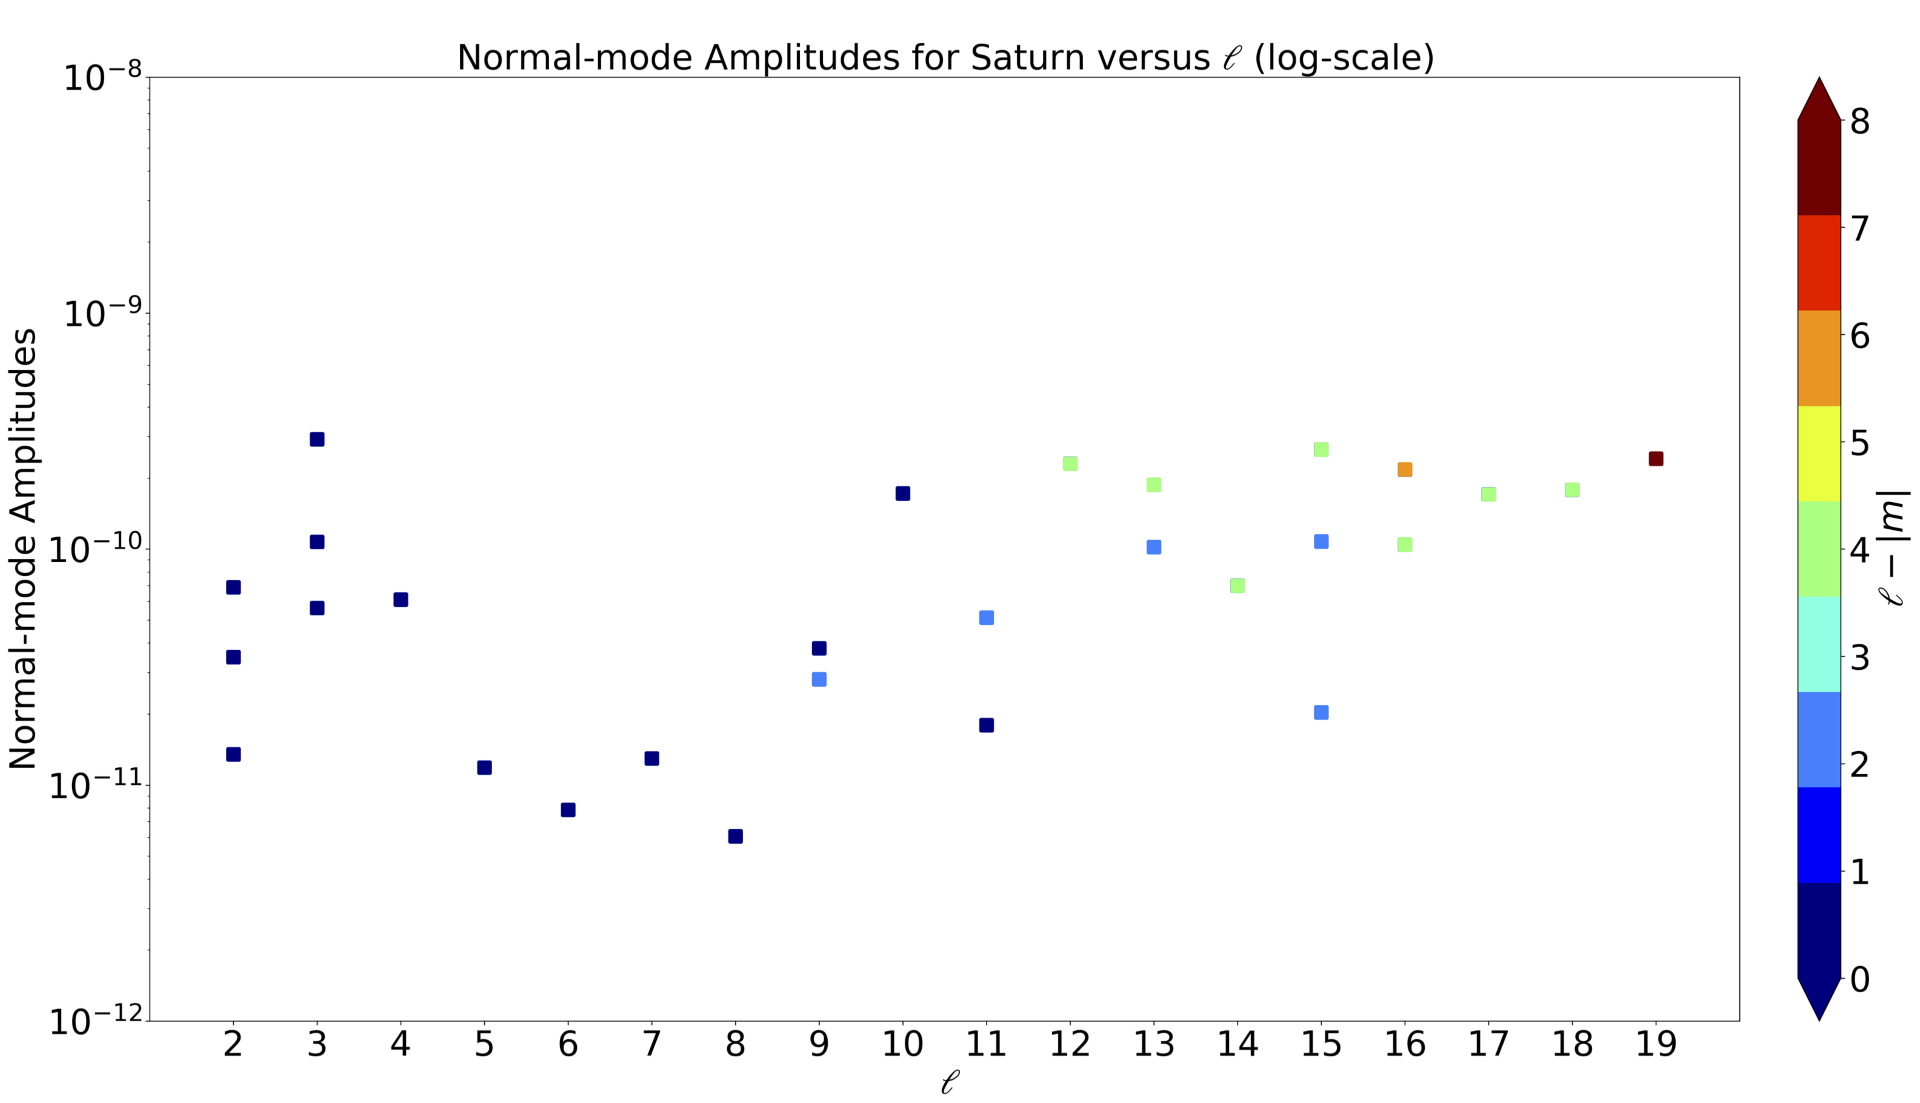
\includegraphics[width=1.0\textwidth]{thumbnail_SaturnAmp_NPROCAVE_VA_082423.png}
\caption{Normal-mode amplitude $\sum_{l=2}^{\infty}\sum_{m=-l}^{l}\bar{C}_{l|m|0}^{'}$ versus angular degree $l$.} \label{fig:my_label}
\end{figure}


\bibliographystyle{plain}\bibliography{reference}

\end{document}